\documentclass{article}
\usepackage{blindtext}
\usepackage{booktabs}
\usepackage[margin=0.25in]{geometry}
\usepackage{subcaption}
\usepackage{graphicx}
\usepackage{caption}
\usepackage{hyperref}
\usepackage{pdflscape}
\usepackage{tikz}


\title{Descriptive Tables and Figures for Municipality Proliferation}

\begin{document}
\maketitle
\tableofcontents
{\footnotesize 
\listoffigures
\listoftables}
\clearpage

\section{Distributions}
\begin{figure}
	\centering
	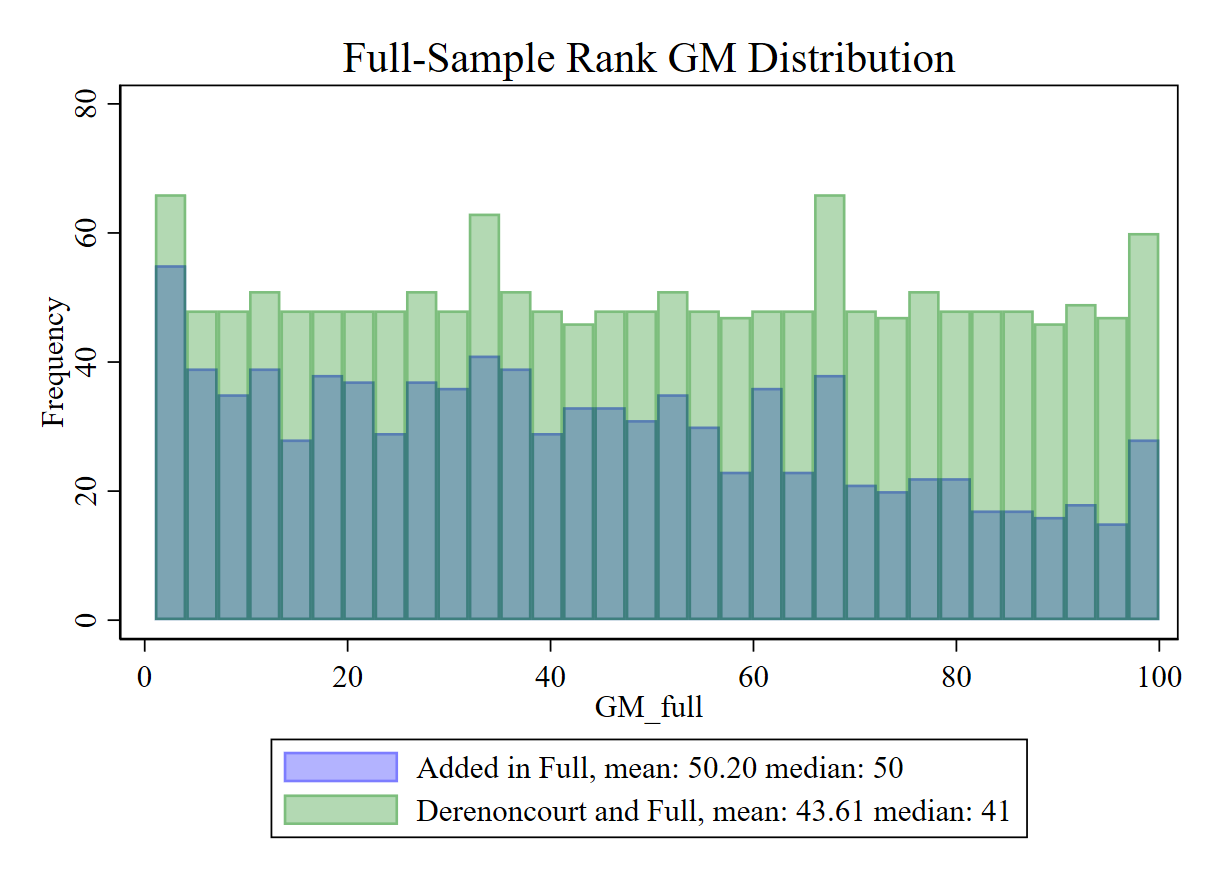
\includegraphics[width=.8\textwidth]{figures/distributions/GM_full.png}
\end{figure}
\clearpage
\begin{figure}
	\centering
	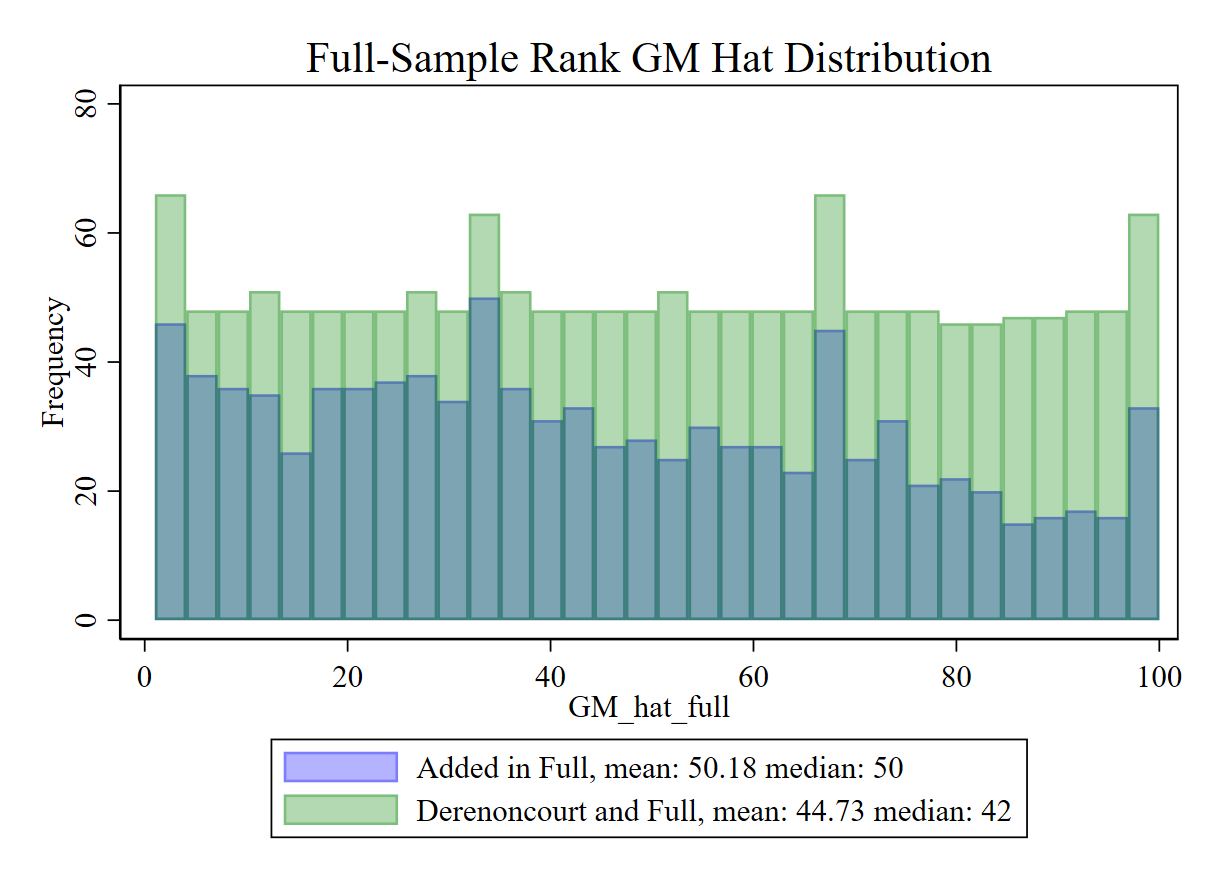
\includegraphics[width=.8\textwidth]{figures/distributions/GM_hat_full.png}
\end{figure}
\clearpage
\begin{figure}
	\centering
	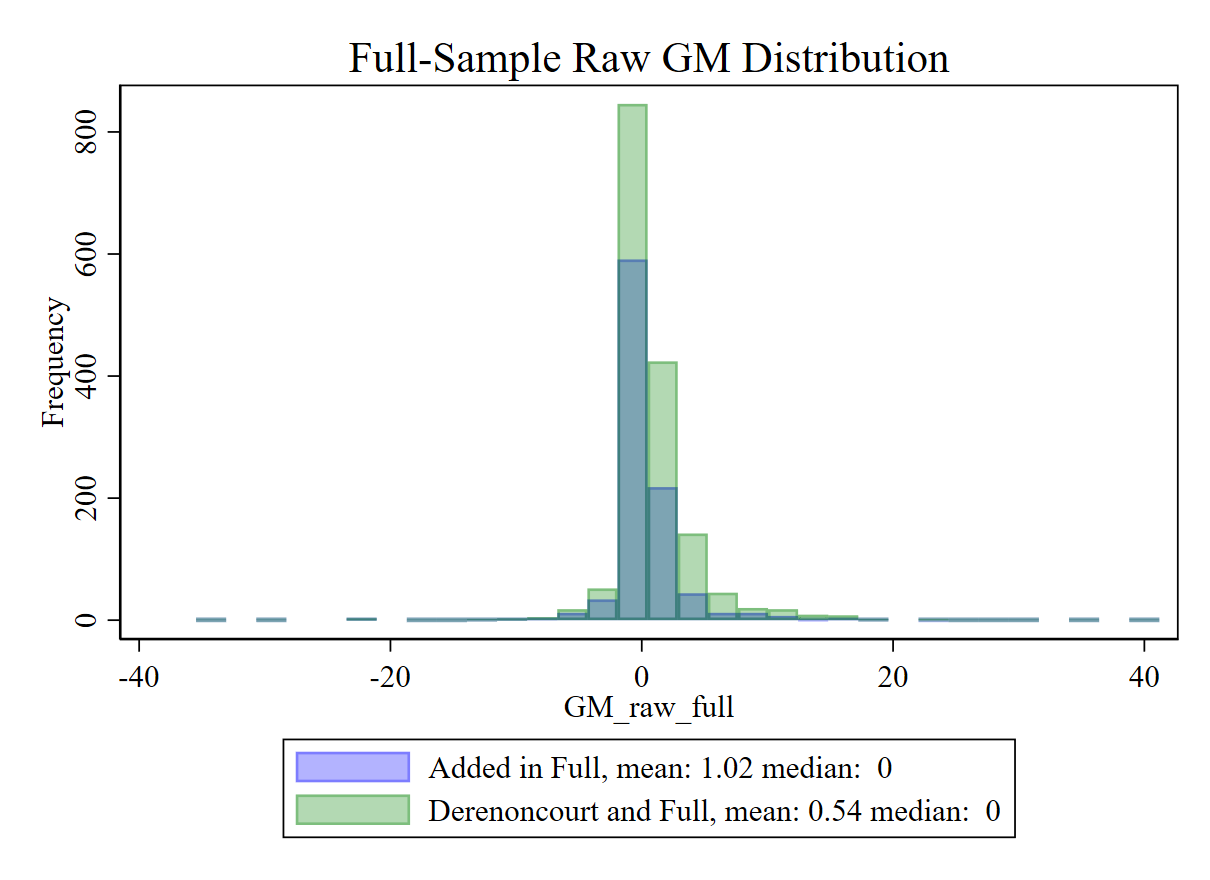
\includegraphics[width=.8\textwidth]{figures/distributions/GM_raw_full.png}
\end{figure}
\clearpage
\begin{figure}
	\centering
	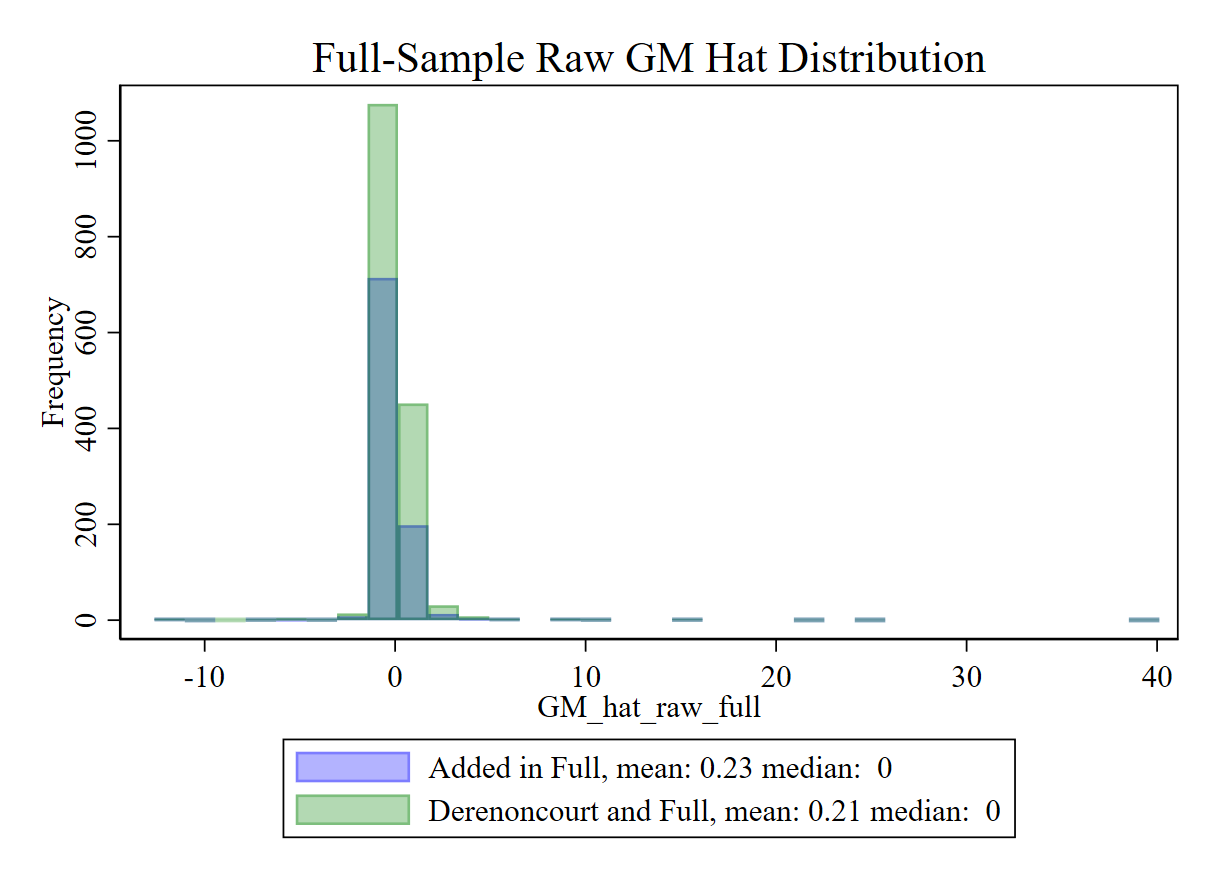
\includegraphics[width=.8\textwidth]{figures/distributions/GM_hat_raw_full.png}
\end{figure}
\clearpage
\begin{figure}
	\centering
	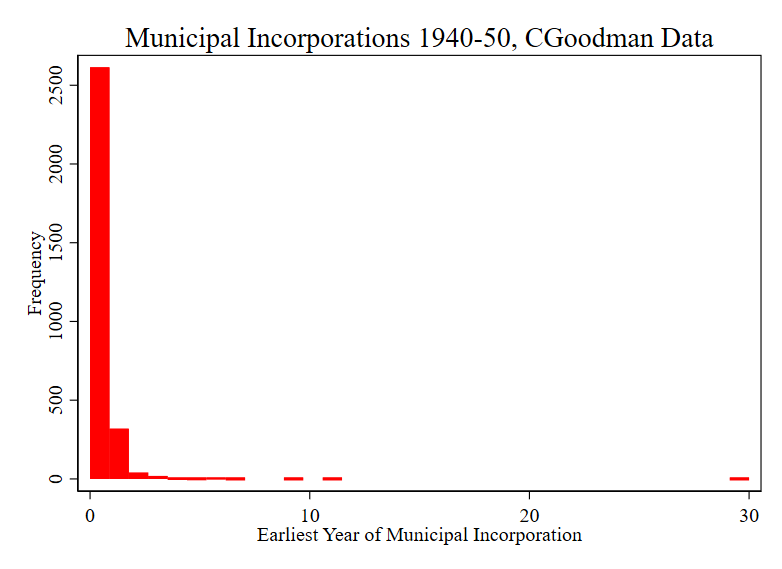
\includegraphics[width=.8\textwidth]{figures/distributions/cgoodman_1940.png}
	\caption{1940-50}
\end{figure}
\clearpage
\begin{figure}
	\centering
	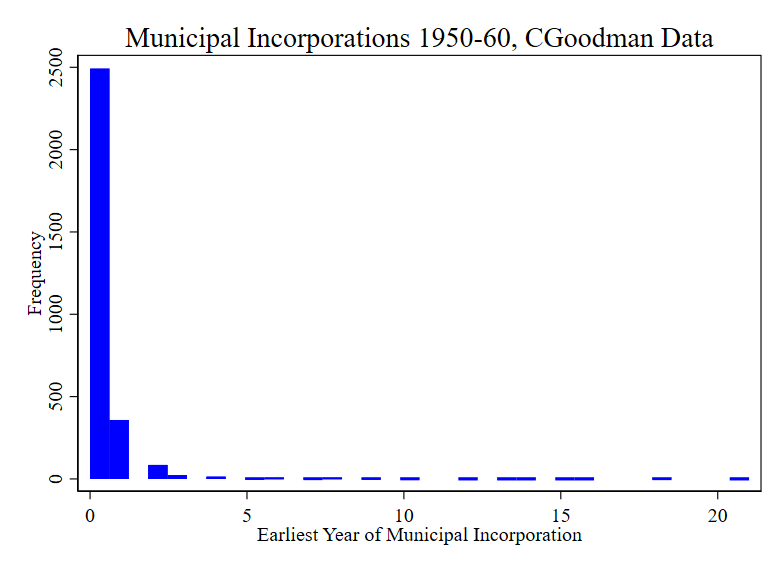
\includegraphics[width=.8\textwidth]{figures/distributions/cgoodman_1950.png}
	\caption{1950-60}
\end{figure}
\clearpage
\begin{figure}
	\centering
	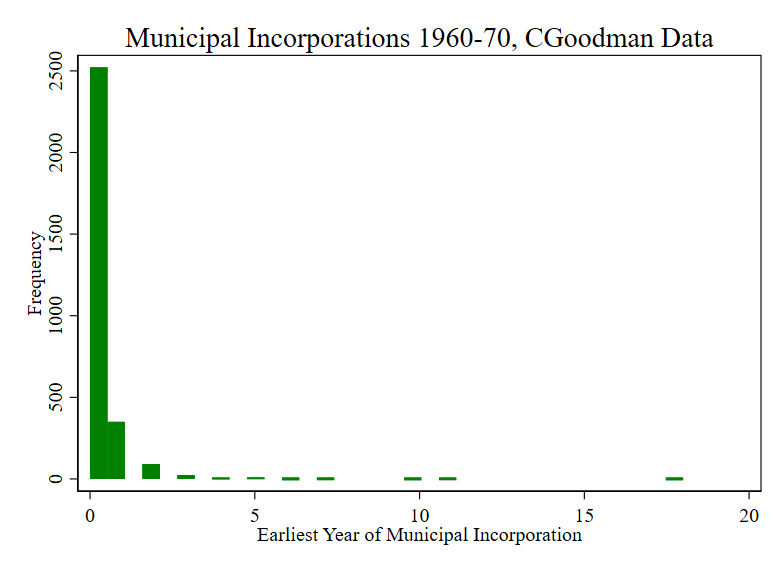
\includegraphics[width=.8\textwidth]{figures/distributions/cgoodman_1960.png}
	\caption{1960-70}
\end{figure}
\clearpage

\section{Jasper vs. Lake Counties}
\clearpage
\begin{figure}
	\centering
	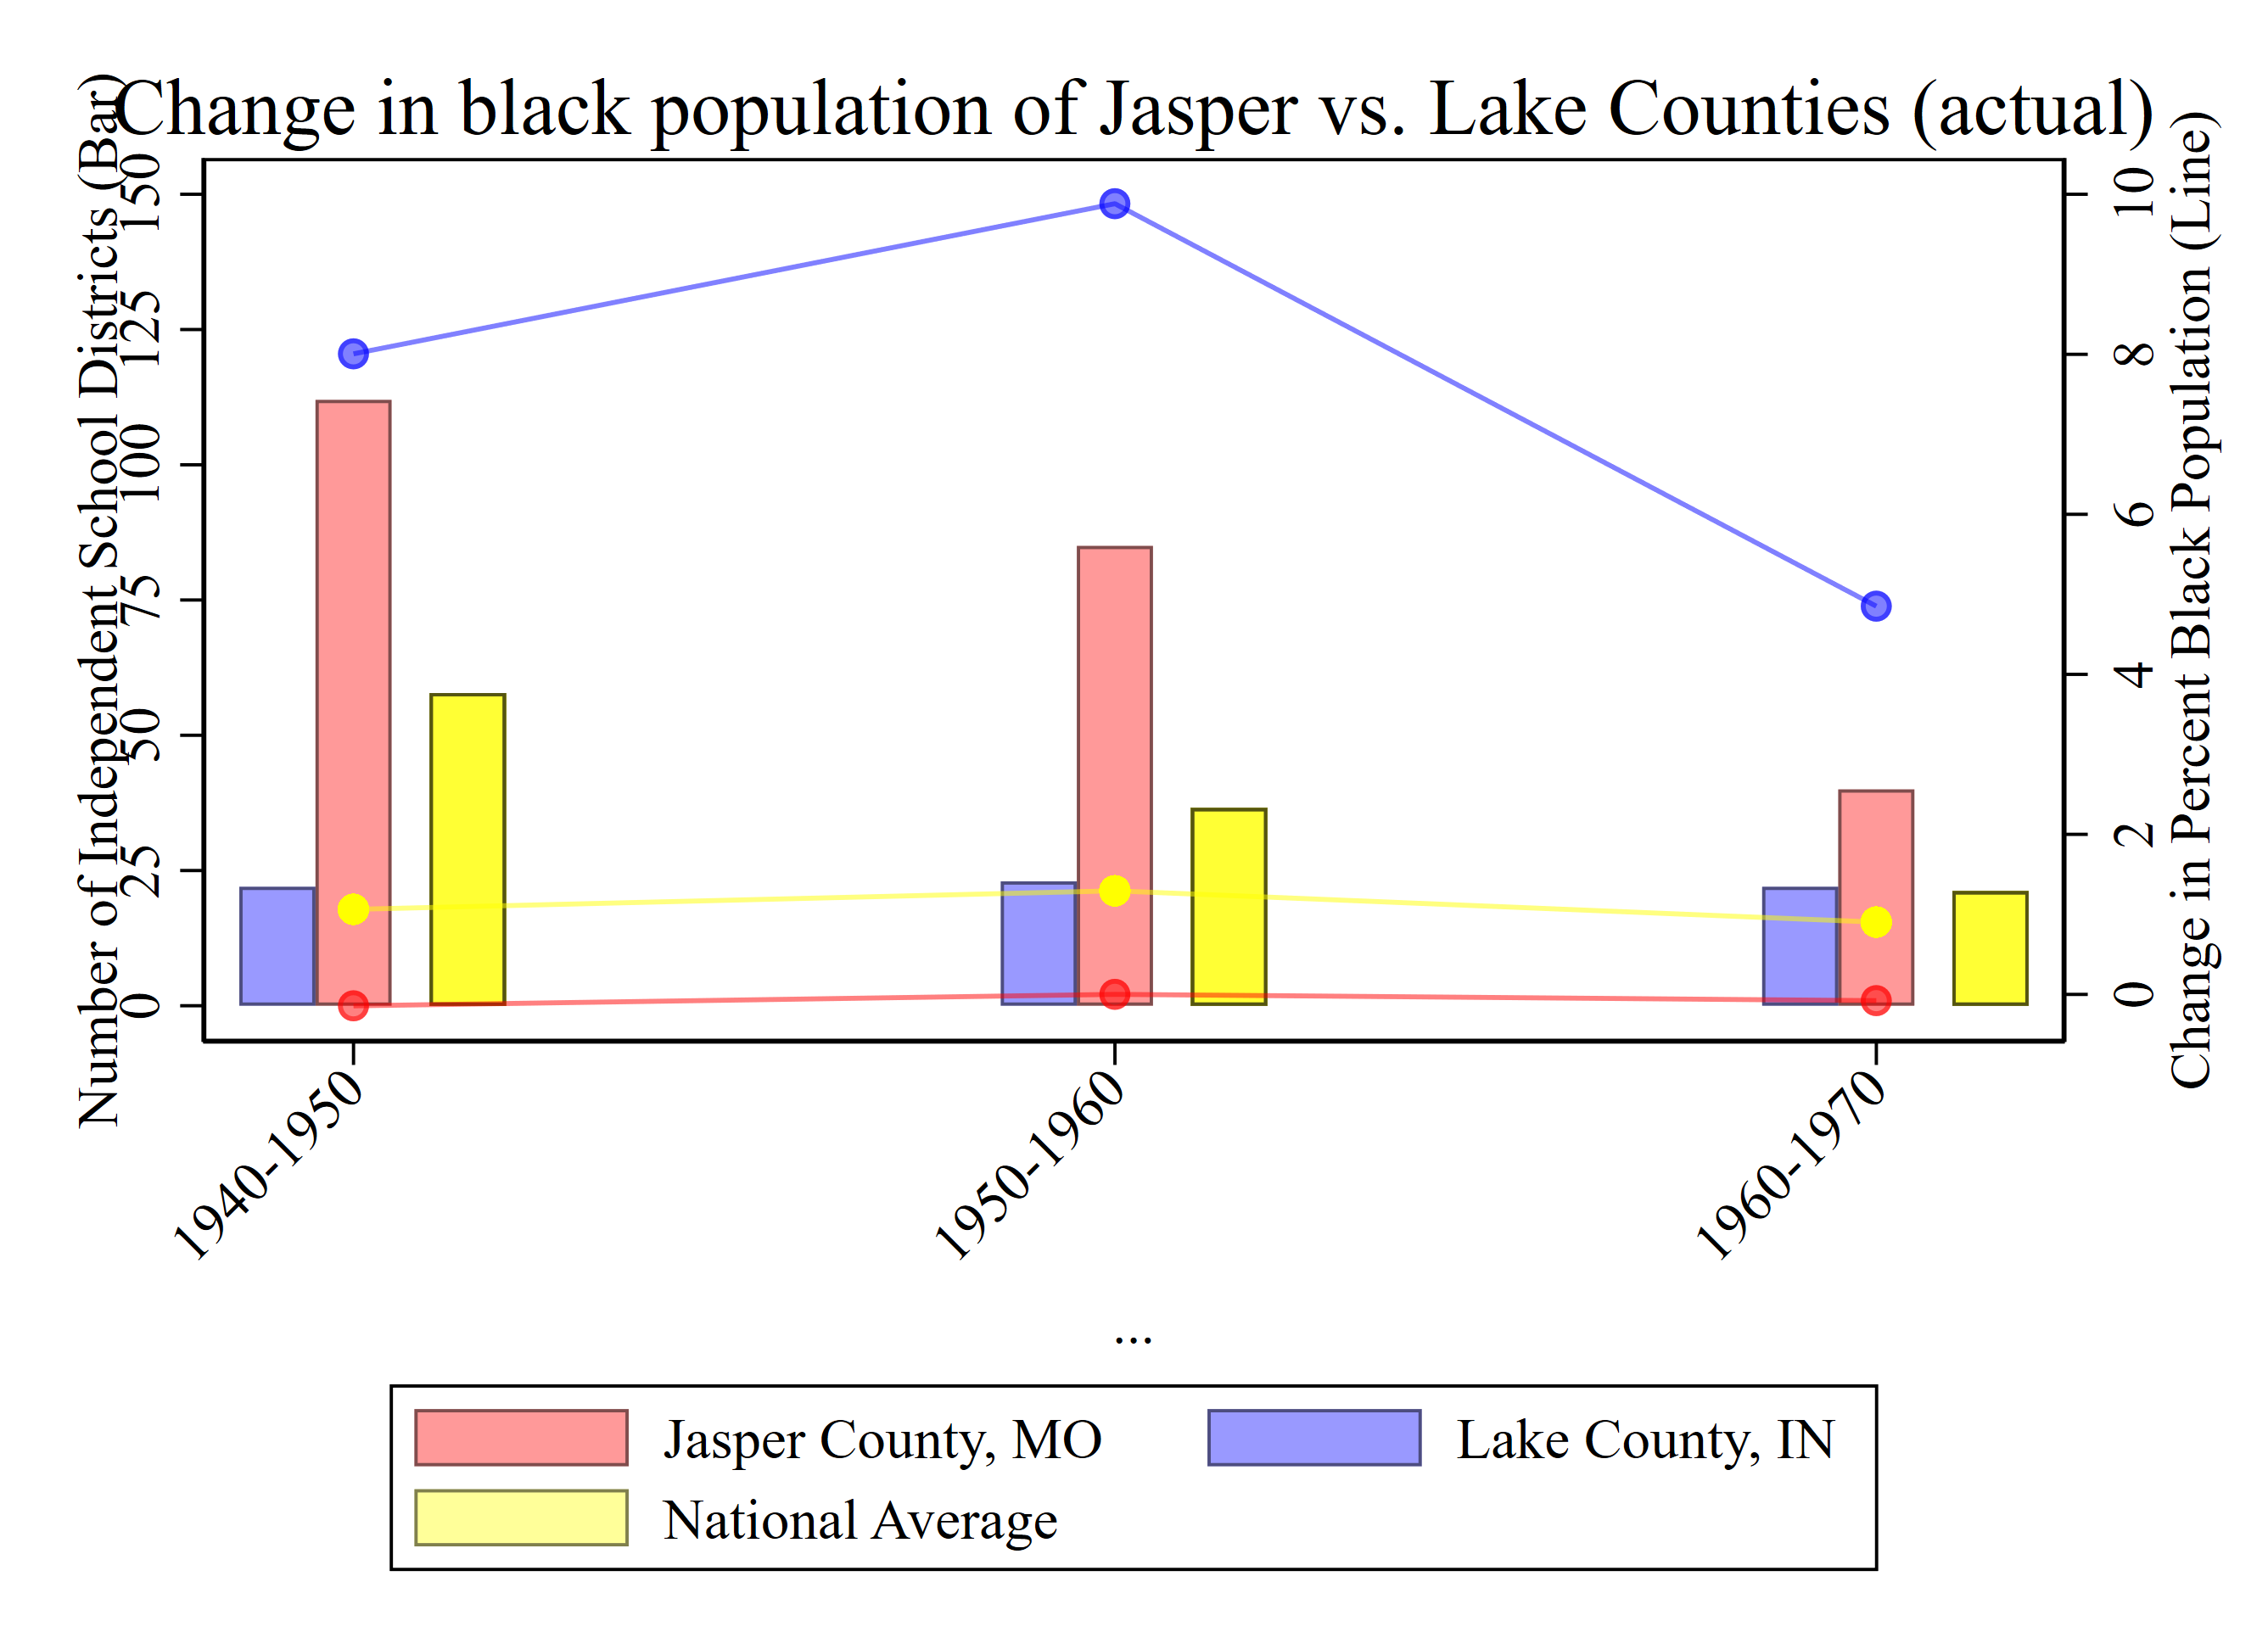
\includegraphics[width=.8\textwidth]{figures/descriptive/comparison.png}
\end{figure}
\clearpage
\begin{figure}
	\centering
	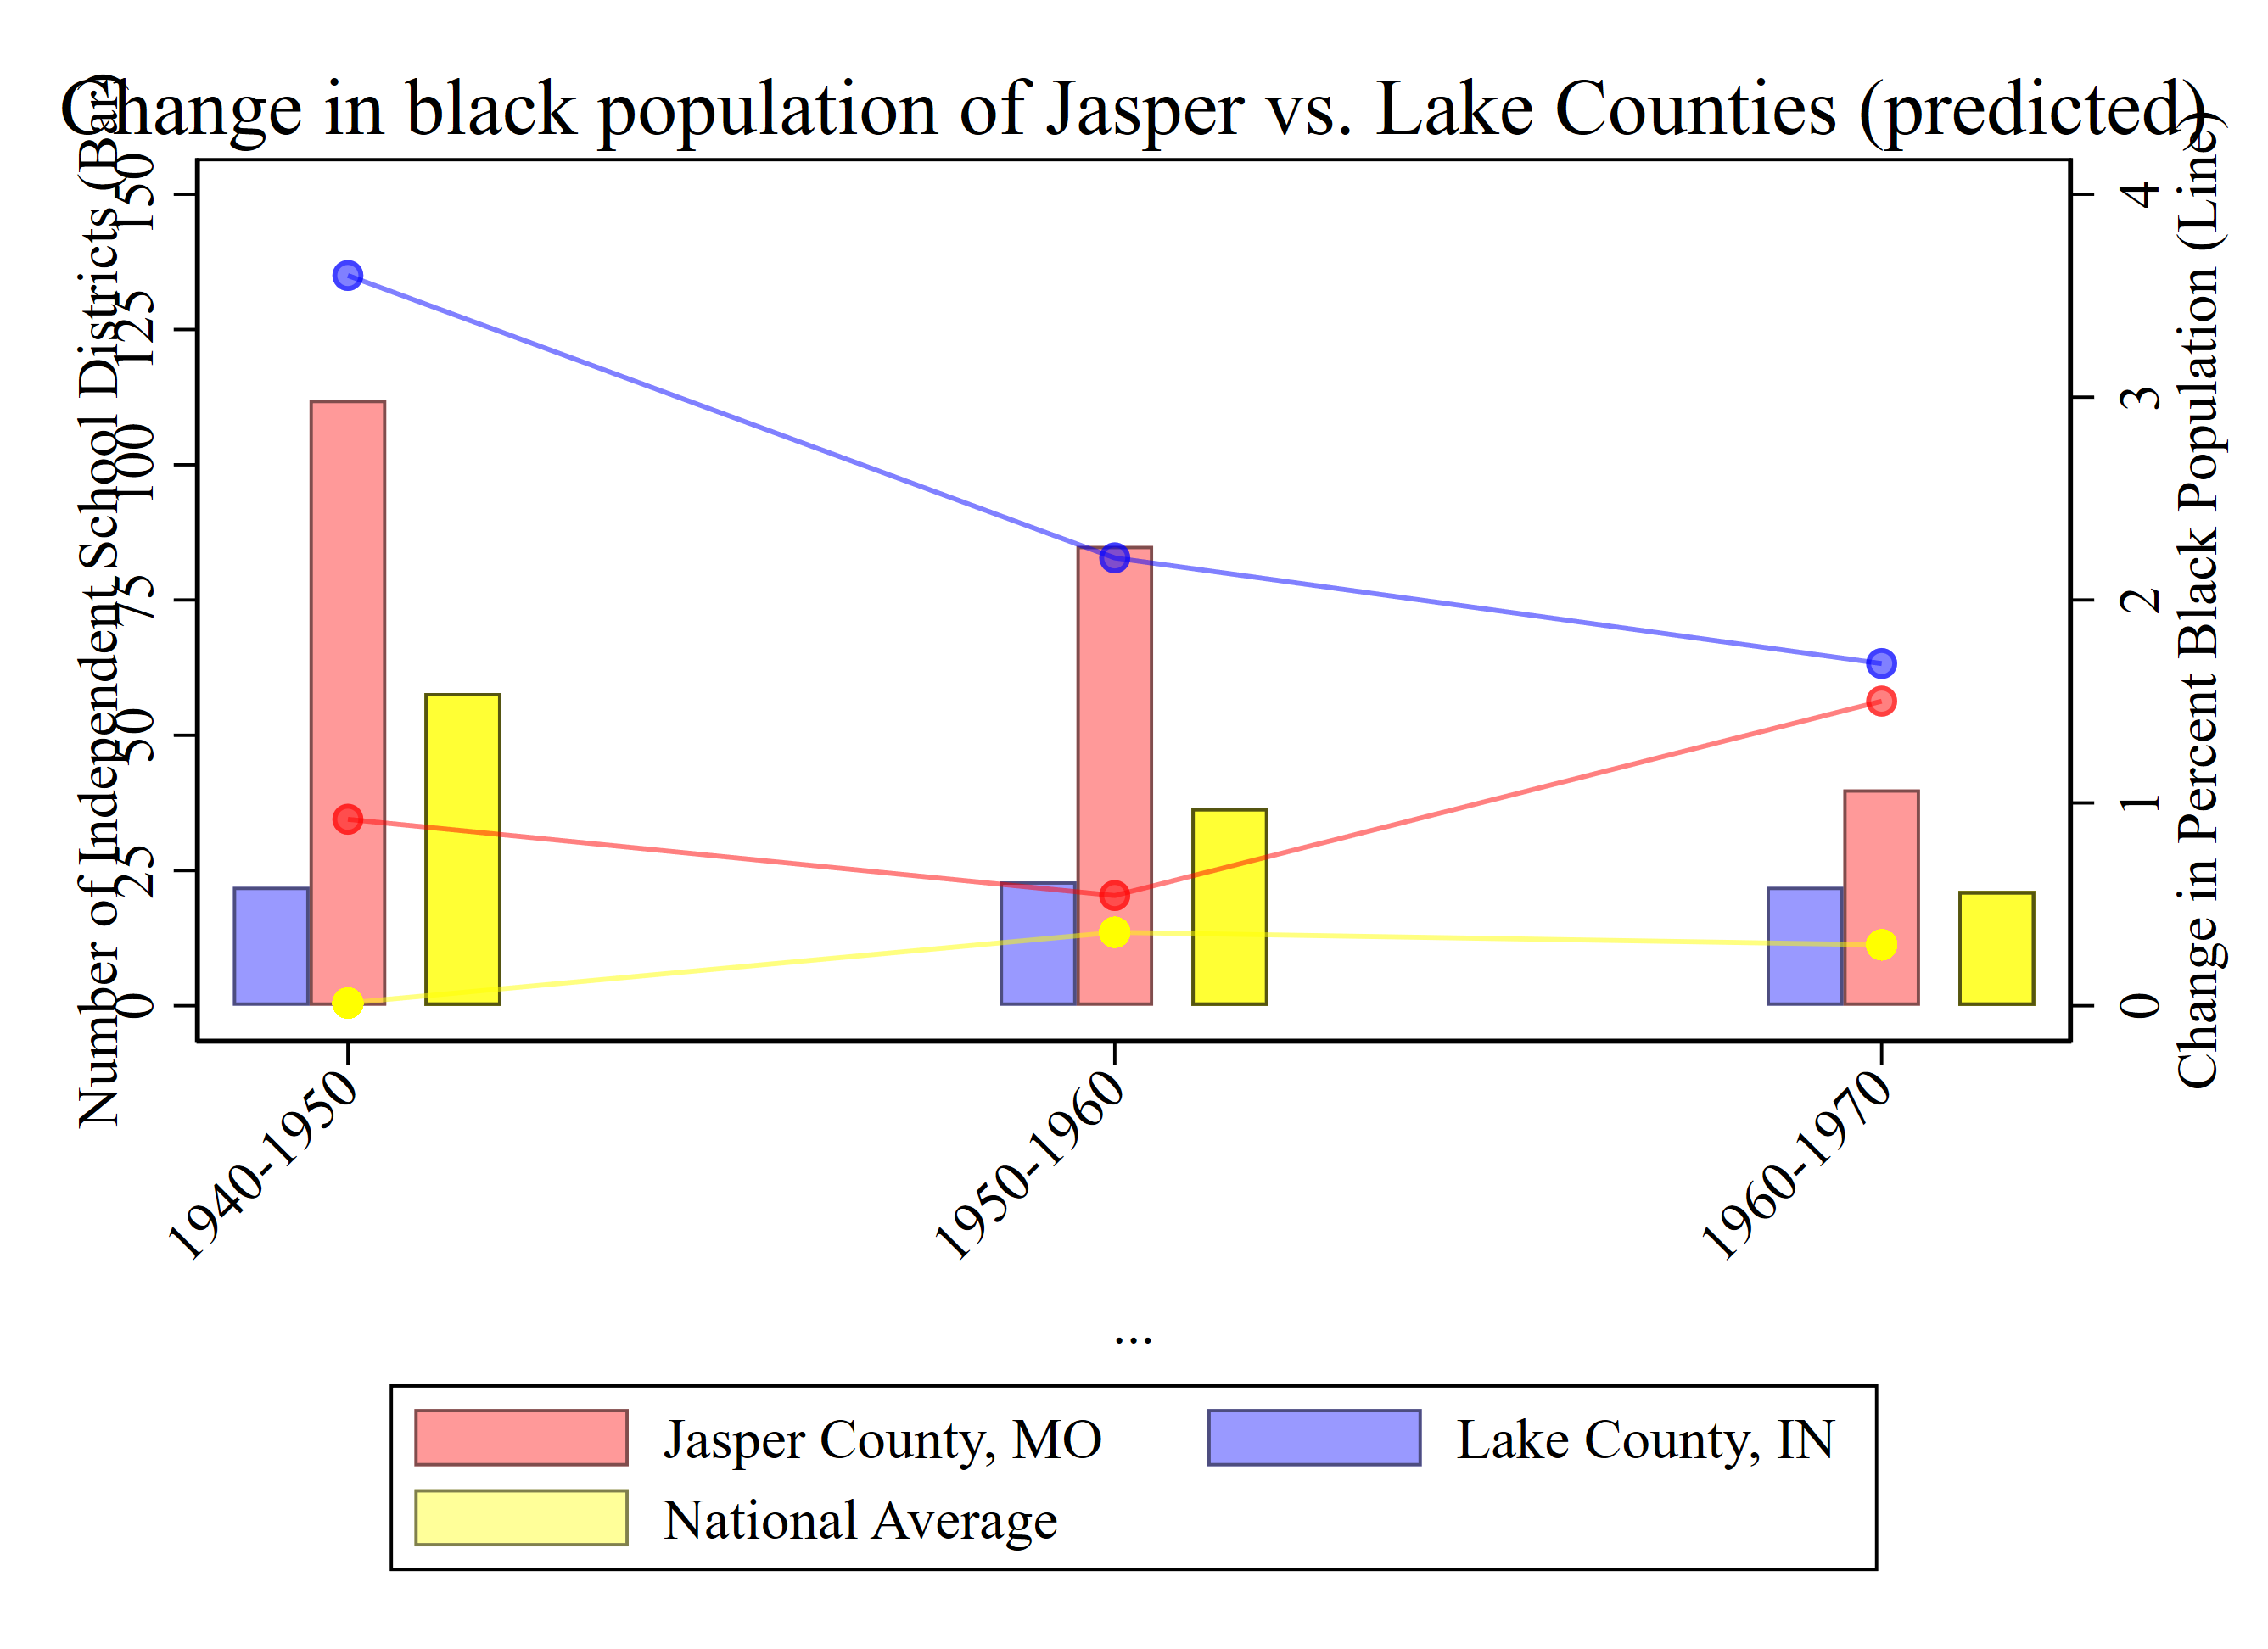
\includegraphics[width=.8\textwidth]{figures/descriptive/comparison_hat.png}
\end{figure}
\clearpage
\section{Goldsmith-Pinkham Table}
\begin{landscape}
{
\def\sym#1{\ifmmode^{#1}\else\(^{#1}\)\fi}
\begin{tabular}{l*{5}{c}}
\toprule
                &\multicolumn{3}{c}{County Counts Outcomes}  &\multicolumn{1}{c}{CGoodman Data}&\multicolumn{1}{c}{Instrument}\\\cmidrule(lr){2-4}\cmidrule(lr){5-5}\cmidrule(lr){6-6}
                &\multicolumn{1}{c}{n\_schdist\_ind\_cz\_pc}&\multicolumn{1}{c}{n\_gen\_subcounty\_cz\_pc}&\multicolumn{1}{c}{n\_gen\_muni\_cz\_pc}&\multicolumn{1}{c}{n\_cgoodman\_cz\_pc}&\multicolumn{1}{c}{GM\_hat\_raw\_pp}\\
\midrule
base\_outcome    &      -0.97***&      -0.22***&      -0.13*  &      -0.14** &              \\
                &     (0.01)   &     (0.04)   &     (0.07)   &     (0.06)   &              \\
\addlinespace
mfg\_lfshare1940 &      -0.35   &       0.38   &       0.25   &       0.19   &       0.08** \\
                &     (0.50)   &     (0.35)   &     (0.21)   &     (0.19)   &     (0.03)   \\
\addlinespace
blackmig3539\_share&     -15.14*  &       3.37   &      -5.64   &      -3.17   &      19.85***\\
                &     (7.94)   &    (11.55)   &     (8.60)   &     (6.28)   &     (5.45)   \\
\addlinespace
pop1940         &      -0.00*  &       0.00   &       0.00*  &       0.00   &       0.00** \\
                &     (0.00)   &     (0.00)   &     (0.00)   &     (0.00)   &     (0.00)   \\
\addlinespace
frac\_land       &     -23.87   &    -107.41** &     -37.28*  &     -33.92*  &      -3.79   \\
                &    (42.93)   &    (47.80)   &    (20.28)   &    (18.05)   &     (6.51)   \\
\addlinespace
reg2            &     -24.50** &     -30.33***&      -7.21** &      -7.50** &       2.31***\\
                &    (11.92)   &     (9.50)   &     (3.60)   &     (3.00)   &     (0.84)   \\
\addlinespace
reg3            &     -26.34*  &      -4.61   &      25.95   &      15.72   &       8.00** \\
                &    (15.10)   &    (21.53)   &    (19.48)   &    (12.48)   &     (3.61)   \\
\addlinespace
reg4            &     -20.49   &     -38.78***&     -10.23   &     -13.09** &      -1.69*  \\
                &    (18.93)   &    (11.90)   &     (7.31)   &     (6.39)   &     (0.96)   \\
\midrule
Observations    &     130.00   &     130.00   &     130.00   &     130.00   &     130.00   \\
\bottomrule
\multicolumn{6}{l}{\footnotesize Standard errors in parentheses}\\
\multicolumn{6}{l}{\footnotesize * p<0.10, ** p<0.05, *** p<0.01}\\
\end{tabular}
}

\clearpage
{
\def\sym#1{\ifmmode^{#1}\else\(^{#1}\)\fi}
\begin{tabular}{l*{5}{c}}
\toprule
                &\multicolumn{3}{c}{County Counts Outcomes}  &\multicolumn{1}{c}{CGoodman Data}&\multicolumn{1}{c}{Instrument}\\\cmidrule(lr){2-4}\cmidrule(lr){5-5}\cmidrule(lr){6-6}
                &\multicolumn{1}{c}{n\_schdist\_ind\_cz\_pc}&\multicolumn{1}{c}{n\_gen\_subcounty\_cz\_pc}&\multicolumn{1}{c}{n\_gen\_muni\_cz\_pc}&\multicolumn{1}{c}{n\_cgoodman\_cz\_pc}&\multicolumn{1}{c}{GM\_hat\_raw\_pp\_totpop}\\
\midrule
base\_outcome    &      -0.97***&      -0.32***&      -0.19** &      -0.19***&              \\
                &     (0.01)   &     (0.05)   &     (0.08)   &     (0.06)   &              \\
\addlinespace
mfg\_lfshare1940 &      -0.19   &      -0.22*  &       0.00   &      -0.01   &       0.01   \\
                &     (0.15)   &     (0.12)   &     (0.07)   &     (0.06)   &     (0.00)   \\
\addlinespace
blackmig3539\_share\_totpop&      -9.67** &      -7.61   &      -2.52   &      -1.95   &       2.65***\\
                &     (4.80)   &     (6.13)   &     (3.54)   &     (2.79)   &     (0.57)   \\
\addlinespace
pop1940         &      -0.00*  &       0.00   &       0.00*  &       0.00   &       0.00** \\
                &     (0.00)   &     (0.00)   &     (0.00)   &     (0.00)   &     (0.00)   \\
\addlinespace
frac\_land       &       5.86   &     -26.32** &     -10.54   &      -8.56   &      -0.87   \\
                &    (14.62)   &    (10.35)   &     (6.66)   &     (5.68)   &     (0.86)   \\
\addlinespace
reg2            &      -2.63   &      -0.74   &       0.14   &       0.18   &       0.19** \\
                &     (2.46)   &     (1.74)   &     (1.13)   &     (0.86)   &     (0.07)   \\
\addlinespace
reg3            &      -5.07   &      -2.24   &       1.88   &      -0.95   &      -0.30   \\
                &     (3.82)   &     (5.13)   &     (5.30)   &     (4.27)   &     (0.24)   \\
\addlinespace
reg4            &      -1.39   &      -9.77***&      -2.27   &      -2.70*  &       0.34***\\
                &     (4.99)   &     (3.50)   &     (1.78)   &     (1.45)   &     (0.10)   \\
\midrule
Observations    &     130.00   &     130.00   &     130.00   &     130.00   &     130.00   \\
\bottomrule
\multicolumn{6}{l}{\footnotesize Standard errors in parentheses}\\
\multicolumn{6}{l}{\footnotesize * p<0.10, ** p<0.05, *** p<0.01}\\
\end{tabular}
}

\clearpage
{
\def\sym#1{\ifmmode^{#1}\else\(^{#1}\)\fi}
\begin{tabular}{l*{5}{c}}
\toprule
                &\multicolumn{3}{c}{County Counts Outcomes}  &\multicolumn{1}{c}{CGoodman Data}&\multicolumn{1}{c}{Instrument}\\\cmidrule(lr){2-4}\cmidrule(lr){5-5}\cmidrule(lr){6-6}
                &\multicolumn{1}{c}{n\_schdist\_ind\_cz\_L0\_pc}&\multicolumn{1}{c}{n\_gen\_subcounty\_cz\_L0\_pc}&\multicolumn{1}{c}{n\_gen\_muni\_cz\_L0\_pc}&\multicolumn{1}{c}{n\_cgoodman\_cz\_L0\_pc}&\multicolumn{1}{c}{GM\_hat\_raw\_pp}\\
\midrule
base\_outcome    &      -0.57***&      -0.07***&      -0.03   &      -0.04   &              \\
                &     (0.06)   &     (0.02)   &     (0.03)   &     (0.03)   &              \\
\addlinespace
mfg\_lfshare     &      -0.27   &       0.31***&       0.16** &       0.12** &       0.07***\\
                &     (0.62)   &     (0.11)   &     (0.07)   &     (0.06)   &     (0.02)   \\
\addlinespace
blackmig3539\_share&     -47.14*  &       5.65   &      -0.60   &       0.06   &      24.38***\\
                &    (25.06)   &     (6.21)   &     (3.97)   &     (3.61)   &     (4.46)   \\
\addlinespace
pop             &       0.00   &      -0.00   &       0.00   &       0.00   &       0.00***\\
                &     (0.00)   &     (0.00)   &     (0.00)   &     (0.00)   &     (0.00)   \\
\addlinespace
frac\_land       &     -27.60   &     -27.47** &      -5.94   &      -6.36   &      -5.84   \\
                &    (54.92)   &    (11.40)   &     (5.01)   &     (4.66)   &     (5.09)   \\
\addlinespace
reg2            &      -6.11   &     -10.49***&      -2.86***&      -2.84***&       1.94***\\
                &    (10.04)   &     (2.88)   &     (0.88)   &     (0.76)   &     (0.60)   \\
\addlinespace
reg3            &       5.52   &      -1.20   &       8.70** &       5.15   &       8.49***\\
                &    (15.28)   &     (5.40)   &     (3.87)   &     (3.65)   &     (2.55)   \\
\addlinespace
reg4            &     -13.23   &      -9.75***&      -2.30   &      -3.60*  &      -0.82   \\
                &    (13.90)   &     (3.62)   &     (2.00)   &     (1.85)   &     (0.74)   \\
\addlinespace
1940.decade     &       0.00   &       0.00   &       0.00   &       0.00   &       0.00   \\
                &        (.)   &        (.)   &        (.)   &        (.)   &        (.)   \\
\addlinespace
1950.decade     &     -68.33***&       1.73   &       1.60   &       0.92   &       1.48***\\
                &    (13.75)   &     (2.12)   &     (0.98)   &     (0.90)   &     (0.39)   \\
\addlinespace
1960.decade     &     -62.96***&       9.21***&       4.06***&       3.54***&       3.65***\\
                &    (12.58)   &     (2.33)   &     (1.00)   &     (0.92)   &     (0.52)   \\
\midrule
Observations    &     390.00   &     390.00   &     390.00   &     390.00   &     390.00   \\
\bottomrule
\multicolumn{6}{l}{\footnotesize Standard errors in parentheses}\\
\multicolumn{6}{l}{\footnotesize * p<0.10, ** p<0.05, *** p<0.01}\\
\end{tabular}
}

\clearpage
{
\def\sym#1{\ifmmode^{#1}\else\(^{#1}\)\fi}
\begin{tabular}{l*{5}{c}}
\toprule
                &\multicolumn{3}{c}{County Counts Outcomes}  &\multicolumn{1}{c}{CGoodman Data}&\multicolumn{1}{c}{Instrument}\\\cmidrule(lr){2-4}\cmidrule(lr){5-5}\cmidrule(lr){6-6}
                &\multicolumn{1}{c}{n\_schdist\_ind\_cz\_L0\_pc}&\multicolumn{1}{c}{n\_gen\_subcounty\_cz\_L0\_pc}&\multicolumn{1}{c}{n\_gen\_muni\_cz\_L0\_pc}&\multicolumn{1}{c}{n\_cgoodman\_cz\_L0\_pc}&\multicolumn{1}{c}{GM\_hat\_raw\_pp\_totpop}\\
\midrule
base\_outcome    &      -0.50***&      -0.10***&      -0.04*  &      -0.04*  &              \\
                &     (0.05)   &     (0.02)   &     (0.02)   &     (0.02)   &              \\
\addlinespace
mfg\_lfshare     &       0.06   &      -0.04   &       0.02   &       0.01   &       0.01***\\
                &     (0.18)   &     (0.03)   &     (0.02)   &     (0.02)   &     (0.00)   \\
\addlinespace
blackmig3539\_share\_totpop&      -0.88   &       4.41*  &       4.23** &       5.02** &       4.26***\\
                &     (4.49)   &     (2.25)   &     (1.78)   &     (1.97)   &     (1.09)   \\
\addlinespace
pop             &      -0.00   &       0.00   &       0.00   &       0.00   &       0.00   \\
                &     (0.00)   &     (0.00)   &     (0.00)   &     (0.00)   &     (0.00)   \\
\addlinespace
frac\_land       &       9.20   &      -7.89***&      -2.37   &      -2.14   &      -0.50   \\
                &    (16.79)   &     (2.65)   &     (1.53)   &     (1.36)   &     (0.53)   \\
\addlinespace
reg2            &      -3.47   &      -0.88** &      -0.58** &      -0.56** &       0.10   \\
                &     (3.15)   &     (0.44)   &     (0.26)   &     (0.24)   &     (0.08)   \\
\addlinespace
reg3            &       6.36*  &       0.70   &       0.47   &      -0.26   &      -0.12   \\
                &     (3.55)   &     (1.39)   &     (0.89)   &     (0.91)   &     (0.30)   \\
\addlinespace
reg4            &      -0.86   &      -3.09***&      -0.86*  &      -1.13** &      -0.49** \\
                &     (4.25)   &     (1.04)   &     (0.52)   &     (0.45)   &     (0.19)   \\
\addlinespace
1940.decade     &       0.00   &       0.00   &       0.00   &       0.00   &       0.00   \\
                &        (.)   &        (.)   &        (.)   &        (.)   &        (.)   \\
\addlinespace
1950.decade     &     -24.16***&       0.53   &       0.67*  &       0.33   &       0.32***\\
                &     (5.48)   &     (0.60)   &     (0.34)   &     (0.31)   &     (0.11)   \\
\addlinespace
1960.decade     &     -20.08***&       2.05***&       1.27***&       1.22***&       0.25** \\
                &     (5.08)   &     (0.62)   &     (0.30)   &     (0.32)   &     (0.12)   \\
\midrule
Observations    &     405.00   &     405.00   &     405.00   &     405.00   &     405.00   \\
\bottomrule
\multicolumn{6}{l}{\footnotesize Standard errors in parentheses}\\
\multicolumn{6}{l}{\footnotesize * p<0.10, ** p<0.05, *** p<0.01}\\
\end{tabular}
}

\clearpage
\end{landscape}

\section{County Comparisons: Overall}

This compares a set of "Treated" and "Control" counties in aggregate. The set is constructed by creating deciles of the county-level recent (1935-39) black migrant share of the 1940 population, then taking the counties with the largest (treated) and smallest (control) 1940-50 change in black population from each decile-census region (10 deciles x 3 regions = 30 possible pairs = 60 possible counties).The 1st and 10th deciles are dropped as the bins are constructed by frequencies, not values, thus their 1940 v2\_blackmig3539\_share values may not actually be that close. Doing this leaves us with 24 pairs/48 counties.

 These tables give summary statistics by decade on the endogenous X variable (GM), instrument (GM\_hat2), control variables (v2\_blackmig3539\_share and mfg\_lfshare), base values of outcome variables (base\_all\_local and base\_schdist\_ind), values of outcome variables (new\_all\_local and new\_schdist\_ind), and county population (countypop).

\foreach \var in {GM, GM_hat2, v2_blackmig3539_share, mfg_lfshare, base_all_local, base_schdist_ind, new_all_local, new_schdist_ind, countypop}{
	\input{tables/comparison_counties/overall_\var.tex}
}
\clearpage
\section{County Comparisons: By Region and blackmig3539\_share bins}
This section compares summary statistics for the 24 decile-census region pairs individually. 
\foreach \reg in {Northeast, Midwest, West}{
	\subsection{\reg Region}
	\foreach \bin in {1,2,3,4,5,6,7,8}{
		\input{tables/comparison_counties/byregXbin_\reg_bin_\bin.tex}
	}
	\clearpage
}

\end{document}